% rubber: set program xelatex
\documentclass[a4paper,12pt]{article}

\usepackage{xltxtra}
\usepackage{amsmath,amsthm,amssymb}

\usepackage[autostyle=true]{csquotes}
\usepackage{polyglossia}
\setmainlanguage{english}
%\setmainlanguage[variant=mono]{greek}
%\setotherlanguage{english}

% Fonts
\setmainfont{CMU Serif}
\setsansfont{CMU Sans Serif}
\setmonofont{CMU Typewriter Text} 


\usepackage[xetex, colorlinks=true, citecolor=blue, linkcolor=blue]{hyperref}

% Diagrams
\usepackage{tikz}
\usetikzlibrary{shapes,arrows}

% Define block styles
\tikzstyle{decision} = [diamond, draw, fill=blue!20, 
    text width=4.5em, text badly centered, node distance=3cm, inner sep=0pt]
\tikzstyle{block} = [rectangle, draw, fill=blue!20, 
    text width=15em, text centered, rounded corners, minimum height=4em]
\tikzstyle{line} = [draw, -latex']
\tikzstyle{cloud} = [draw, ellipse,fill=red!20, node distance=3cm,
    minimum height=2em]

\usepackage{mathtools}

% Source code listings
\usepackage{listings}
\usepackage{color}
\usepackage{matlab-prettifier}
\lstdefinestyle{My-Matlab}
{
  style               = MatlabBaseStyle@mlpr,
  basicstyle          = \color{black}\ttfamily\small,
  mllastelementstyle  = \color{black}                    ,
  mlkeywordstyle      = \color[RGB]{000,000,255}         ,
  mlcommentstyle      = \color[RGB]{034,139,034}         ,
  mlstringstyle       = \color[RGB]{160,032,240}         ,
  mlsyscomstyle       = \color[RGB]{178,140,000}         ,
  mlsectiontitlestyle = \commentStyle@mlpr      \bfseries,
  mlsharedvarstyle    = \color[RGB]{000,163,163}         ,
  mlplaceholderstyle  = \mleditorphstyle,
}



\title{
\normalfont \normalsize 
\textsc{University of Burgundy \\ 
Image Analysis
, MSCV 2018} \\
[10pt] 
\rule{\linewidth}{0.5pt} \\[6pt] 
\huge Sparse Visual Tracking \\
\rule{\linewidth}{2pt}  \\[10pt]
}
\author{Ioannis Tsagkatakis \\ Hassan Saeed}
\date{\normalsize \today}

\begin{document}

\maketitle
\noindent


\section{Introduction}
Mathematical transformations are applied to signals to obtain further information from that signal that is not readily available in the raw signal. There are a number of transformations that can be applied, among which the Fourier transforms are probably by far the most popular.

\subsection{Why Wavelet Transform }
The Fourier transform gives the frequency components (spectral) exists in the signal. But, when the time-localization of spectral components is needed, a transform giving the TIME-FREQUENCY representation of signal is needed. This is in short, if we take the Fourier transform over the whole time axis, we cannot tell at what instant a particular frequency rises. The wavelet transform is a transform which gives this sort of information. There are other transforms which give this information too, like Short-time Fourier transform (STFT) uses a sliding window to find spectrogram, which gives the information of both time and frequency. But still another problem exists: The length of window limits the resolution in frequency. Wavelet transform seems to be a solution to the problem above.

\subsection{Discrete Wavelet Transform}
The discrete wavelet transform (DWT), provides sufficient information both for analysis and synthesis of the original signal, with a significant reduction in the computation time. The DWT is considerably easier to implement when compared to the Continuous Wavelet Transform (CWT). The main idea is the same as it is in the Continuous Wavelet Transform. A time-scale representation of a digital signal is obtained using digital filtering techniques. The CWT is a correlation between a wavelet at different scales and the signal with the scale (or the frequency) being used as a measure of similarity. The continuous wavelet transform is computed by changing the scale of the analysis window, shifting the window in time, multiplying by the signal, and integrating over all times. In the discrete case, filters of different cutoff frequencies are used to analyze the signal at different scales. The signal is passed through a series of high pass filters to analyze the high frequencies, and it is passed through a series of low pass filters to analyze the low frequencies. The resolution of the signal, which is a measure of the amount of detail information in the signal, is changed by the filtering operations, and the scale is changed by up sampling and down sampling operations. Down sampling a signal corresponds to reducing the sampling rate, or removing some of the samples of the signal. Up sampling a signal corresponds to increasing the sampling rate of a signal by adding new samples to the signal.

\begin{figure}[t]
        \centering
        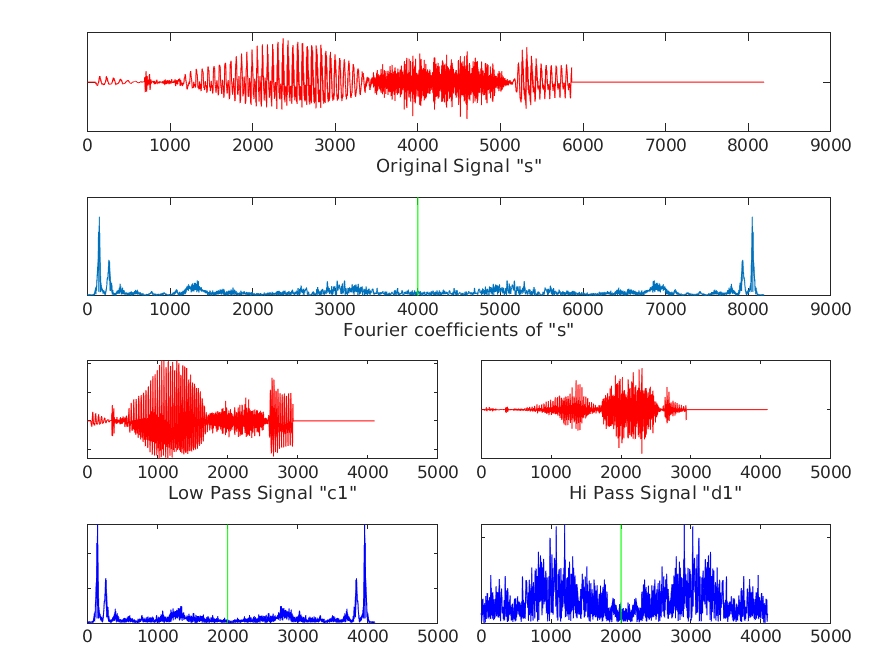
\includegraphics[width=8cm]{../Results/demo_1D_composition}
        \caption{Wavelet Composition of 1D signal}
		\label{fig:demo1}
\end{figure}


\subsection{Wavelet Analysis (Decomposition}
The procedure starts with passing the signal through a half band digital low pass filter with impulse response. A half band low pass filter removes all frequencies that are above half of the highest frequency in the signal. For example, if a signal has a maximum of 500 Hz component, then half band low pass filtering removes all the frequencies above 250 Hz. After passing the signal through a half band low pass filter, half of the samples can be eliminated according to the Nyquist’s rule, since the signal now has a highest frequency of p/2 radians instead of p radians (if p is original highest frequency of signal). Simply discarding every other sample will down sample the signal by two, and the signal will then have half the number of points. The scale of the signal is now doubled. Here, the low pass filtering removes the high frequency information, but leaves the scale unchanged. Only the down sampling process changes the scale. The DWT analyzes the signal at different frequency bands with different resolutions by decomposing the signal into a coarse approximation and detail information. DWT employs two sets of functions, called scaling functions and wavelet functions, which are associated with low pass and high pass filters, respectively. 


\begin{figure}[t]
        \centering
        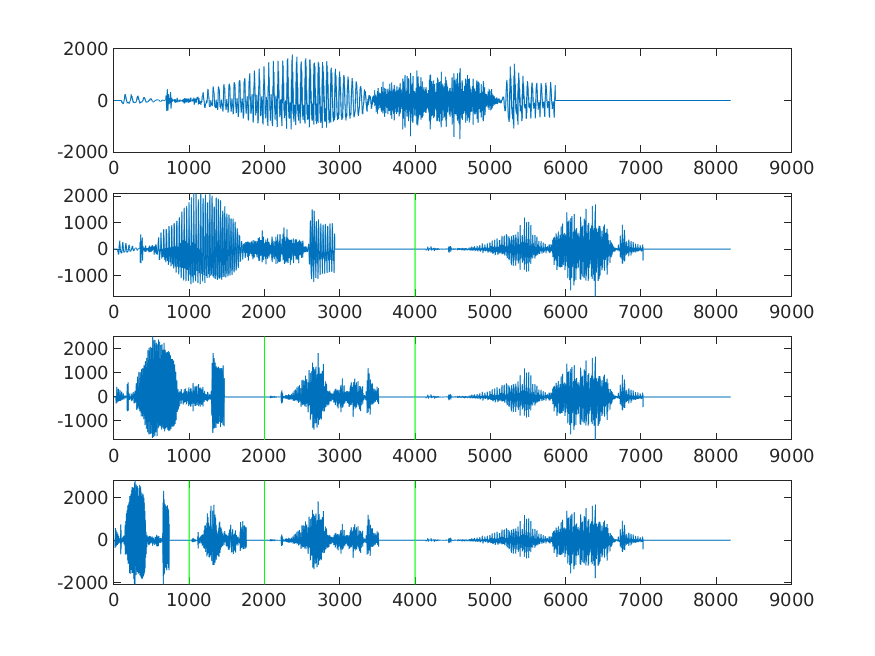
\includegraphics[width=8cm]{../Results/demo_1D_deconposition.png}
        \caption{Wavelet decomposition of 1D signal}
		\label{fig:demo2}
\end{figure}

The decomposition of the signal into different frequency bands is simply obtained by successive high pass and low pass filtering of the time domain signal. The original signal x[n] is first passed through a half band high pass filter g[n] and a low pass filter h[n]. After the filtering, half of the samples can be eliminated. This constitutes one level of decomposition. This decomposition can be continued to multi level using the coarse approximation as input to next level.


The decomposition process can be seen in a block diagram in Figure~\ref{fig:wave1}.

\begin{figure}[t]
        \centering
        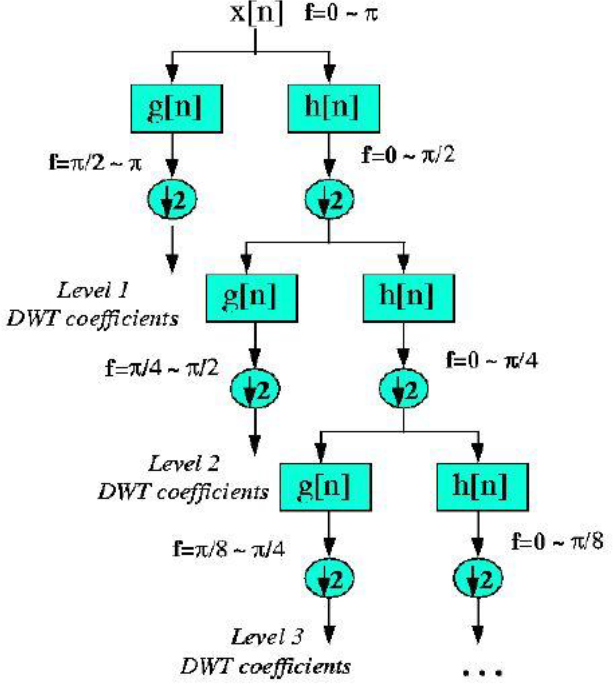
\includegraphics[width=8cm]{diagram.png}
        \caption{Wavelet Decomposition of 1D signal}
		\label{fig:wave1}
\end{figure}

In figure~\ref{fig:demo1} created by matlab script \texttt{demo\_1D\_composition.m} the ...




\section{Wavelet Synthesis (Reconstruction)}
The reconstruction of original signal from the wavelet coefficients is the reverse process of the decomposition. As we get the wavelet coefficients, we need to up sample the coefficients which halves the scale of the signal. After the signal is up sampled we apply low pass and high pass filters to the up sampled signal to get the perfect reconstructed signal.



\section{2D DWT}
For images, an algorithm similar to the one-dimensional case is possible for two-dimensional wavelets. This kind of two-dimensional DWT leads to a decomposition of approximation coefficients at level $j$ in four components: the approximation at level $j+1$, and the details in three orientations (horizontal, vertical, and diagonal). The schematic diagram of 2D wavelet analysis (decomposition) is as shown in Figure~\ref{fig:wave2}.

\begin{figure}[tb]
        \centering
        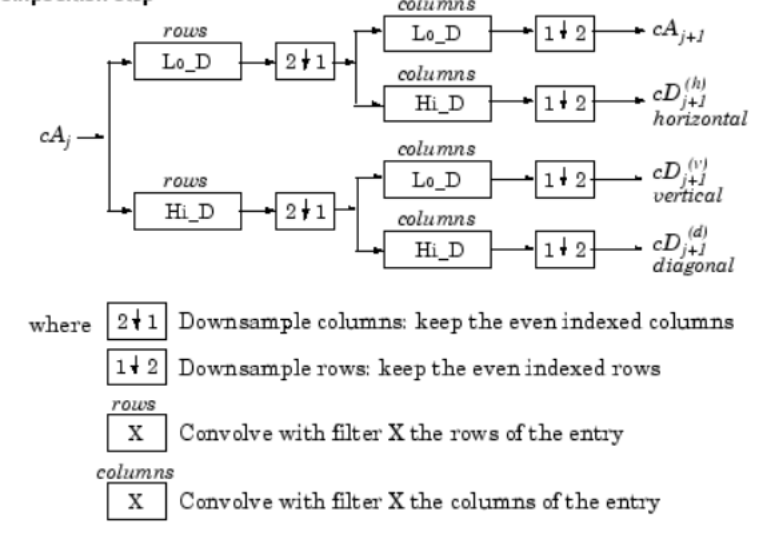
\includegraphics[width=8cm]{diagram2.png}
        \caption{Schematic diagram of 2D DWT decomposition}
		\label{fig:wave1}
\end{figure}

\noindent The algorithm is simple
\begin{enumerate}
\item Apply $1D$ wavelet transform to each row
\item Apply $1D$ wavelet transform to each column of the result
\end{enumerate} 

\noindent The components of a wavelets transform ... to directional edges of the image. This is demonstrated on Figure~\ref{fig:rubik} on page \pageref{fig:rubik}.

\begin{figure}[bt]
        \centering
        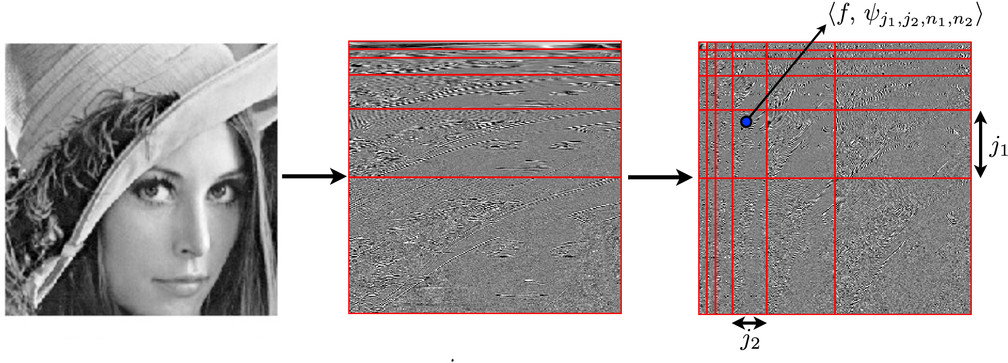
\includegraphics[width=8cm]{explain2D.png}
        \caption{2D Decompositionusing wavelets}
		\label{fig:wave2}
\end{figure}
\noindent Figure~\ref{fig:wave2} outlines the process.


\begin{figure}[tb]
        \centering
        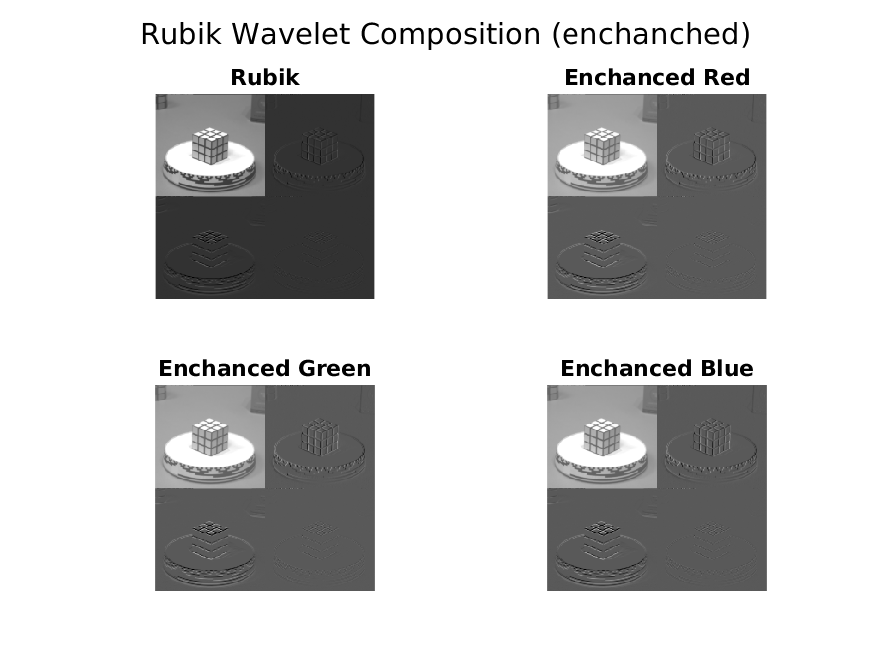
\includegraphics[width=8cm]{../Results/Rubik_Ench.png}
        \caption{Enchanced 2D to make edges more visible}
		\label{fig:rubik}
\end{figure}

\FloatBarrier

\section {Denoising}
The data sets of many scientific experiments are corrupted with noise, either because of the data acquisition process, or because of environmental effects. A first pre-processing step in analyzing such datasets is denoising, that is, estimating the unknown signal of interest from the available noisy data. There are several different approaches to denoise signals and images. Generally smoothing removes high frequency and retains low frequency (with blurring). De-blurring increases the sharpness signal features by boosting the high frequencies, whereas denoising tries to remove whatever noise is present regardless of the spectral content of a noisy signal. Wavelet transforms enable us to represent signals with a high degree of sparsity. This is the principle behind a non-linear wavelet based signal estimation technique known as wavelet denoising. Wavelet denoising attempts to remove the noise present in the signal while preserving the signal characteristics, regardless of its frequency content.

\section{Study of a Harr Wavelet Filter}
The code this report as well as the results can be found in  github at \url{https://github.com/jtsagata/sparce_waveltes}.

$$
H_o(z) = \frac{1}{\sqrt{2}}\left( 1 + z^{-1}\right)
$$


\begin{figure}[t]
        \centering
        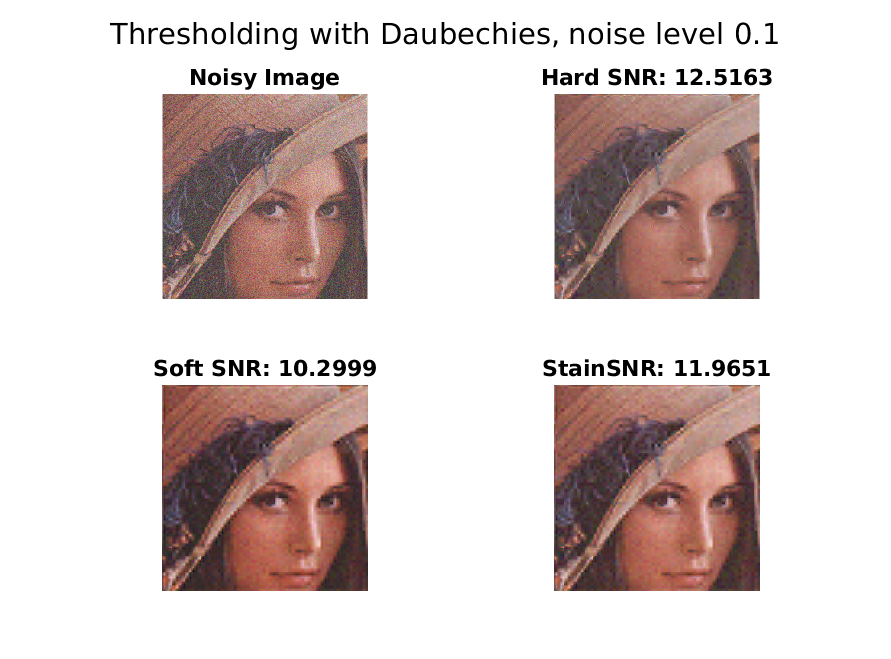
\includegraphics[width=8cm]{../Results/leana_threshold.png}
        \caption{Threshold functions and denoising results}
		\label{fig:threshold}
\end{figure}


\begin{figure}[t]   
        \centering
        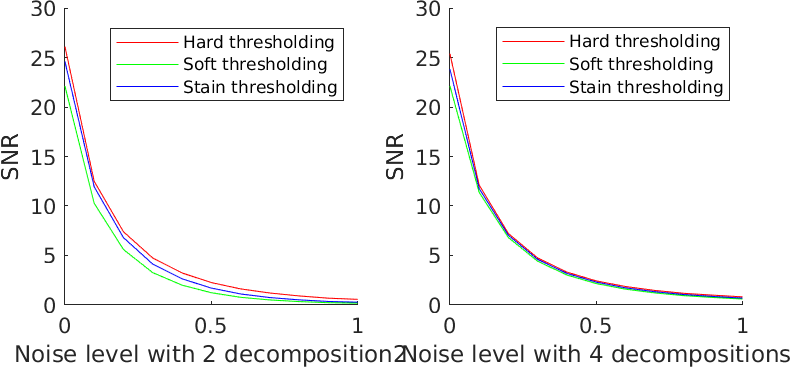
\includegraphics[width=8cm]{../Results/noise_levels.png}
        \caption{Effect of th}
		\label{fig:noiselevel}
\end{figure}


\section{Denoising}
\begin{figure}[t]
        \centering
        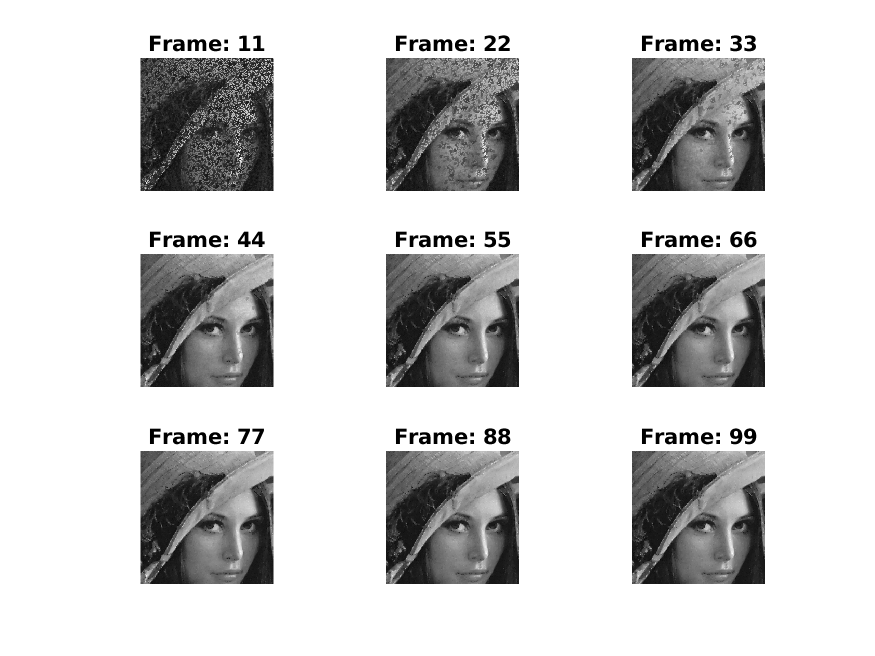
\includegraphics{../Videos/lena_primal_frames.png}
        \caption{Give me a name} 
		\label{fig:denoise_video}
\end{figure}


\section{Inpaining}
\begin{figure}[t]
        \centering
        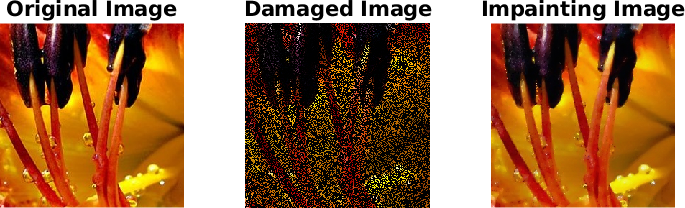
\includegraphics{../Results/Inpainting_pdual_flowers_evolution.png}
        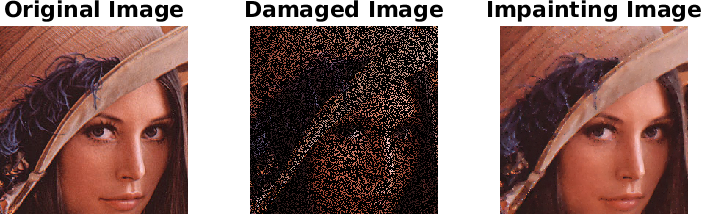
\includegraphics{../Results/Inpainting_pdual_lena_evolution.png}
        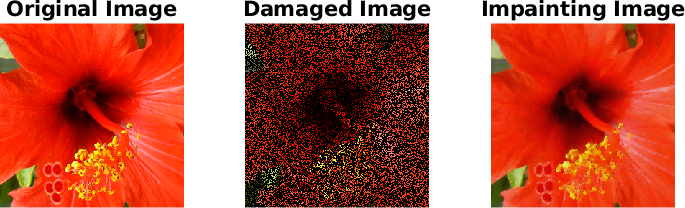
\includegraphics{../Results/Inpainting_pdual_hibiscus_evolution.png}
		\label{fig:evolve1}
\end{figure}

\begin{figure}[t]
        \centering
        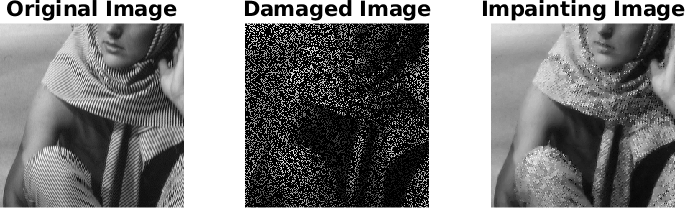
\includegraphics{../Results/Inpainting_pdual_barb_evolution.png}
        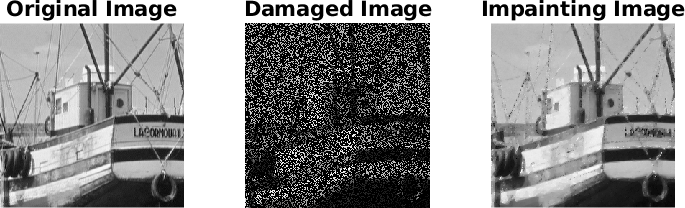
\includegraphics{../Results/Inpainting_pdual_boat_evolution.png}
        \caption{Give me a name} 
		\label{fig:evolve2}
\end{figure}


\begin{figure}[t]
        \centering
        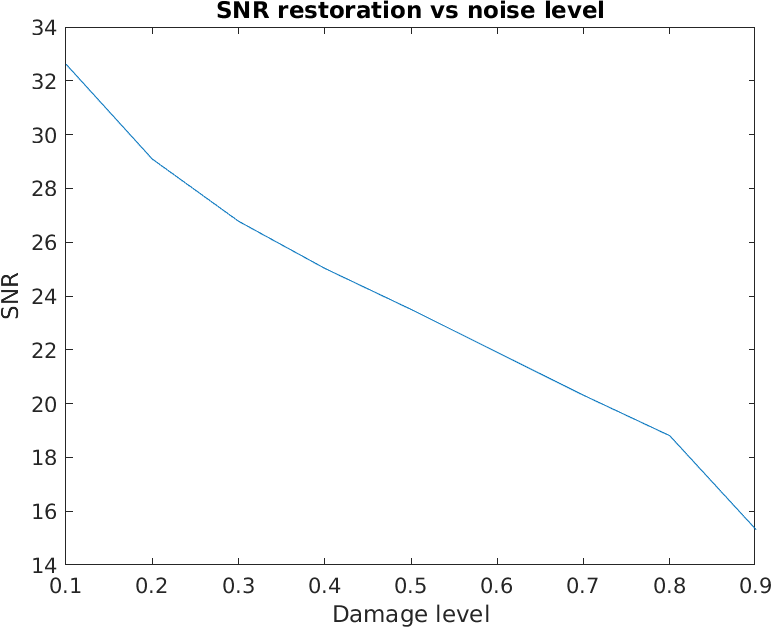
\includegraphics{../Results/Inpainting_lena_noise_vs_SNR.png}
        \caption{Give me a name} 
		\label{fig:nvssnr}
\end{figure}

\FloatBarrier
\section{Matlab code}
The file \texttt{getThreshold.m} calculates the theshold value for the threshold operations.
\lstinputlisting[style=My-Matlab]{../Code/getThreshold.m}

\vspace{18pt}
\noindent The file \texttt{Denoising.m} performs denoising operation on an image.
\lstinputlisting[style=My-Matlab]{../Code/Denoising.m}

\vspace{18pt} 
\noindent The file \texttt{ImpaintingPrimalDual.m} performs inpaining using regularization with primal-dual tone varation.
\lstinputlisting[style=My-Matlab]{../Code/ImpaintingPrimalDual.m}


\end{document}
